% {{{1 PRELUDE
\documentclass{beamer}

% Packages
\usepackage[francais]{babel}
% \usepackage[english]{babel}
\usepackage[utf8]{inputenc}
\usepackage[T1]{fontenc}
\usepackage{amsmath,amssymb}

% Custom commands
\newcommand{\R}{\mathbb{R}}

\usetheme{Frankfurt}

\AtBeginSection[]
{
    \begin{frame}
        \frametitle{Sommaire}
        \tableofcontents[currentsection, hideothersubsections]
    \end{frame}
}

\title[Lissage adaptatif de nuages de points]{Lissage adaptatif de nuages de
    points}
\author[MEYRON Jocelyn]{MEYRON Jocelyn\\\scriptsize{Encadré par:\\
        ATTALI Dominique, GIPSA-lab\\
        MÉRIGOT Quentin, CEREMADE, Université Paris-Dauphine}}
\institute{GIPSA-lab}
\date{5 juin 2015}

\begin{document}

\begin{frame}
    \titlepage
\end{frame}

\begin{frame}
    \tableofcontents
\end{frame}

% {{{1 INTRODUCTION
\section{Introduction}

\begin{frame}[allowframebreaks]
    \frametitle{Introduction}
    % \framesubtitle{Introduction}

    Quoi?
    \begin{itemize}
        \item Objet étudié: nuage de points
        \item Facile à acquérir: scanner 3D
        \item Création de modèles plus complets: maillages
        \item Problème: erreur de mesure, présence de bruit $ \to $ lissage
    \end{itemize}

    \begin{figure}
        \centering
        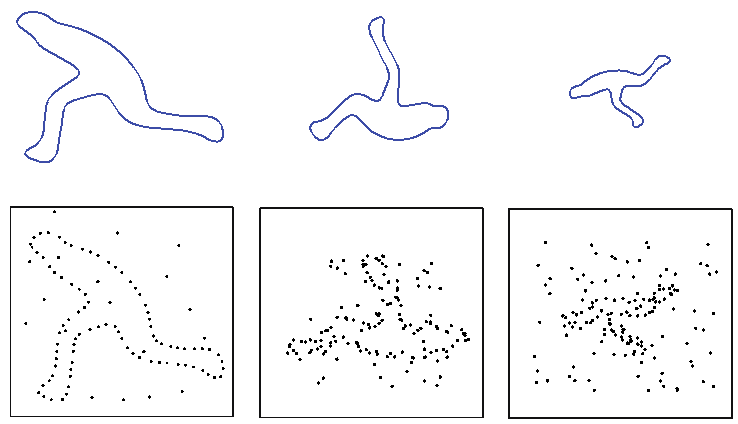
\includegraphics[scale=0.25]{img/noise-2d}
        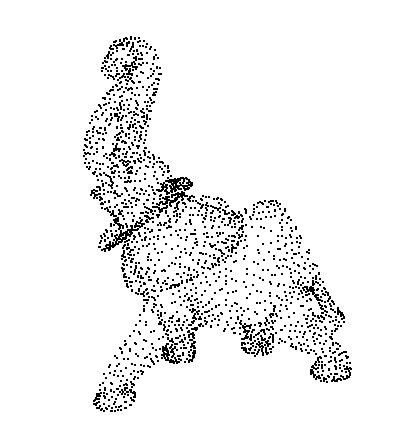
\includegraphics[scale=0.2]{img/elephant-point-cloud}
        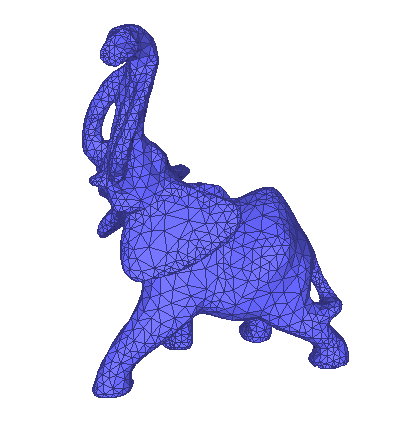
\includegraphics[scale=0.2]{img/elephant-mesh}
    \end{figure}

    \newpage
    Comment?
    \begin{itemize}
        \item Outils de traitement d'image inaccessibles: Transformée de
            Fourier...
        \item Pas de paramétrisation: voisins?
        \item Autre idée: flot de courbure moyenne
    \end{itemize}

    \begin{figure}
        \centering
        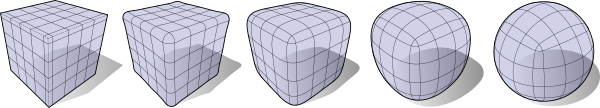
\includegraphics[scale=0.3]{img/mean-curvature-flow-cube}
    \end{figure}
\end{frame}

\begin{frame}
    \frametitle{Introduction}
    % \framesubtitle{Flot de courbure moyenne}

    Flot de courbure moyenne:
    \begin{itemize}
        \item Faire évoluer une surface en bougeant chaque point dans la
            direction de la normale et d'une quantité égale à la
            courbure moyenne en ce point
        \item Équivalent à minimiser l'aire de la surface
        \item Propriétés lissantes
        \item Problème: surface inconnue $ \to $ uniquement échantillons
    \end{itemize}

    \begin{figure}
        \centering
        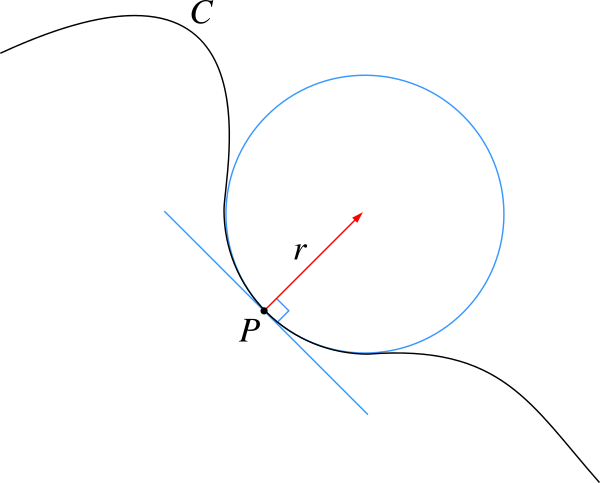
\includegraphics[scale=0.25]{img/osculating-circle}
        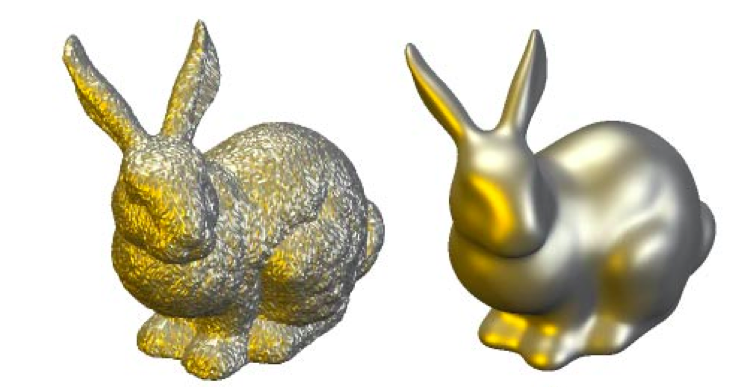
\includegraphics[scale=0.22]{img/mean-curvature-flow-rabbit}
    \end{figure}
\end{frame}

\begin{frame}
    \frametitle{Introduction}
    % \framesubtitle{Comment?}

    \begin{itemize}
        \item Approximation de l'aire de la surface: union de boules
        \item Minimisation d'une énergie $ E : \R^{dN} \to \R $: descente de gradient
        \item Calcul du gradient: différentiation automatique
            \begin{itemize}
                \item Gradients: variation de l'énergie quand on bouge chacun
                    des points
                \item Surcharge du type de nombre, opérations et fonctions
                    usuelles, dérivation composée
            \end{itemize}
        \item Autres énergies: aire du bord, pondération, anisotrope
    \end{itemize}
\end{frame}

\begin{frame}
    \frametitle{Introduction}
    % \framesubtitle{Objectifs}

    \emph{Objectifs}
    \begin{enumerate}
        \item Flot de courbure moyenne sur des nuages de points
        \item Flot de courbure moyenne anisotrope: remplacer l'union des boules
            par une union de polyèdres convexes
    \end{enumerate}

    \emph{Applications:}
    \begin{enumerate}
        \item Estimation de courbure moyenne
        \item Lissage / Débruitage
    \end{enumerate}
\end{frame}

% \begin{frame}
%     \frametitle{Introduction}
%     % \framesubtitle{Quelques notions}

%     \begin{definition}[Offset d'un nuage de points]
%         Le $r$-offset d'une nuage de points $ P \subseteq \mathbb{R}^d $ est
%         défini par:
%         $$ P^r = \bigcup_{p \in P} B(p, r) $$
%     \end{definition}

%     \begin{definition}[$\epsilon$-échantillon]
%         Pour une hypersurface $ S $, on dit que $ P \subseteq \mathbb{R}^d $ est
%         un $\epsilon$-échantillon de $ S $ si:
%         $$ \bigcup_{p \in P} B(p, \epsilon) \subseteq S $$
%     \end{definition}
% \end{frame}

% \begin{frame}[allowframebreaks]
%     \frametitle{Introduction}
%     % \framesubtitle{Résultats théoriques}

%     \begin{theorem}[Approximation de l'aire d'une hypersurface]
%         Soit une hypersurface $ S $ de $ \mathbb{R}^d $ et $ P $ un
%         $\epsilon$-échantillon de $ S $, alors:
%         $$ | \frac{Vol^d(P^r)}{2r} - Vol^{d-1}(S) | \leq \frac{\epsilon^2}{2r^2} +
%         O(\frac{\epsilon^4}{r^3}) + O(r^2) $$
%     \end{theorem}

%     \begin{theorem}[Gradient de l'aire]
%         Si $ A = Vol^d(P^r) $ alors en notant $ \nabla_{p_i} A $ la limite
%         suivante:
%         $$ \lim\limits_{\epsilon \to 0} \frac{A(p_1, \ldots, p_{i-1}, p_i + \epsilon
%             \delta p_i, p_{i+1}, \ldots, p_N) - A(p_1, \ldots, p_N)}{\epsilon} $$
%         On a:
%         $$ \nabla_{p_i} A = \int_{B} \frac{x - p_i}{||x - p_i||} dx $$
%         où $ B = \partial B(p_i, r) \cap V(p_i, P) $.
%     \end{theorem}

%     \begin{theorem}[Approximation de la courbure moyenne]
%         Soit une hypersurface $ S $ de $ \mathbb{R}^d $ et soit $ P $ un
%         $\epsilon$-échantillon de $ S $, on a:
%         $$ \nabla_p A \approx 2 r \vec{\kappa}(p) Vol(V(p, P) \cap
%         M) $$
%     \end{theorem}
% \end{frame}

% {{{1 2D
\section{Cas 2D}

\subsection{Problème}
\begin{frame}
    \frametitle{Problème}
    % \framesubtitle{Flot de courbure moyenne}

    Flot de courbure moyenne sur des nuages de points: descente de gradient
    \begin{itemize}
        \item Calcul de l'énergie $ E $ volume (ou périmètre du bord) de l'union de boules
        \item Calcul du gradient
        \item Déplacement des points (Euler explicite): $ p'_i = p_i - \tau \nabla E (p_i) $ où $
            \tau $ est une constante
    \end{itemize}

    \begin{figure}
        \centering
        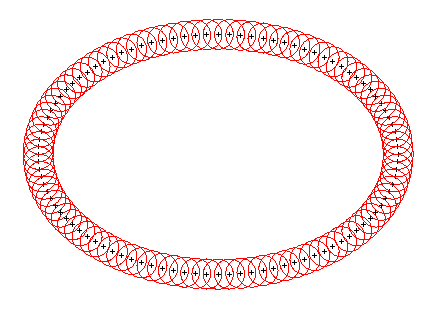
\includegraphics[scale=0.28]{img/ellipse-balls-15}
    \end{figure}
\end{frame}

\begin{frame}
    \frametitle{Calcul du volume}
    % \framesubtitle{Flot de courbure moyenne}

    Diagramme de Voronoi avec \texttt{CGAL}
    \begin{figure}
        \centering
        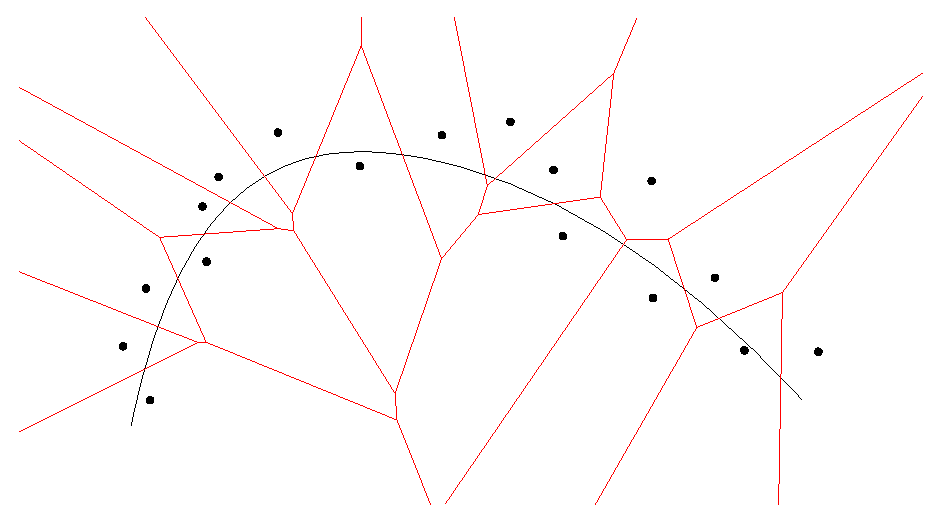
\includegraphics[scale=0.28]{img/voronoi-curve-2d}
        \hfill
        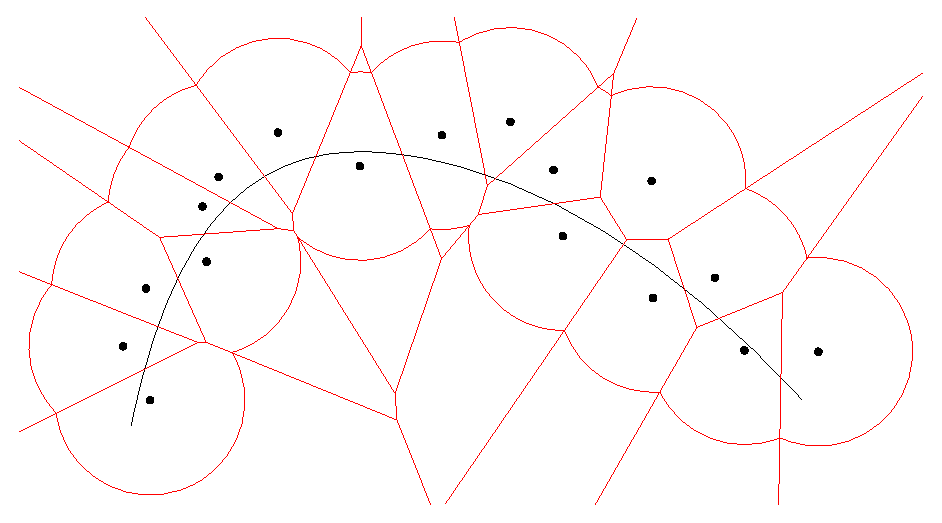
\includegraphics[scale=0.28]{img/voronoi-offset-2d}
    \end{figure}

    Alors:
    $$ E \left( \bigcup_p B(p, r) \right) = \sum_p E(V(p, P) \cap B(p, r)) $$
\end{frame}

\subsection{Estimation de courbure moyenne}
\begin{frame}
    \frametitle{Estimation de courbure moyenne}
    % \framesubtitle{Exemples}

    Exemples: courbure d'une ellipse
    \begin{figure}
        \centering
        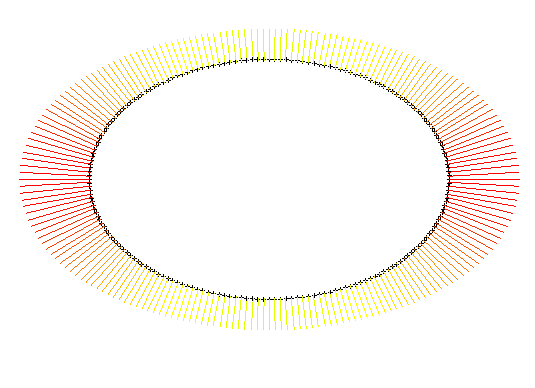
\includegraphics[scale=0.3]{img/curvature-ellipse-200-15-area}
        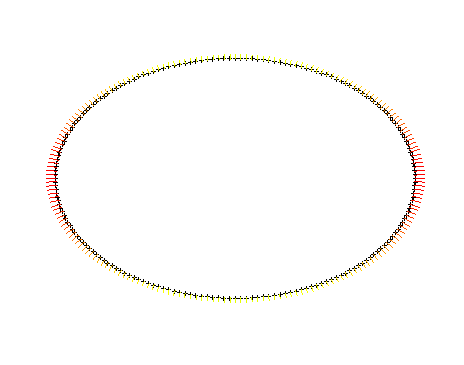
\includegraphics[scale=0.3]{img/curvature-ellipse-200-15-perimeter}
        \caption{E = Aire / E = Périmètre du bord}
    \end{figure}
\end{frame}

\subsection{Flot de courbure moyenne}
\begin{frame}
    \frametitle{Flot de courbure moyenne}
    % \framesubtitle{Exemples}

    Exemples: flot d'une ellipse bruitée
    \begin{figure}
        \centering
        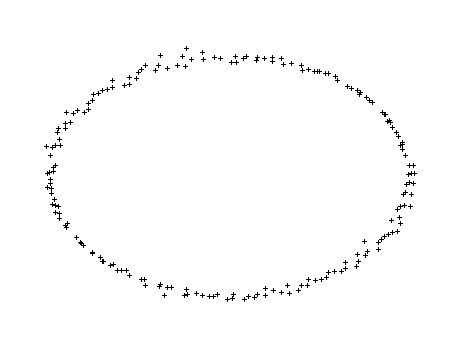
\includegraphics[scale=0.22]{img/ellipse-200-noised-var-1-area}
        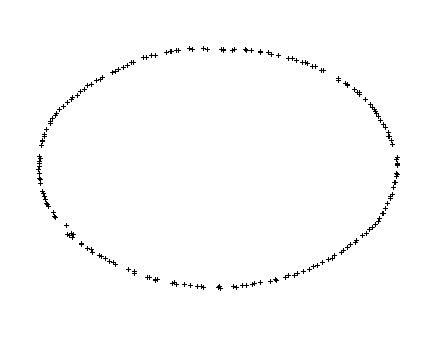
\includegraphics[scale=0.22]{img/ellipse-noised-area-5-01}

        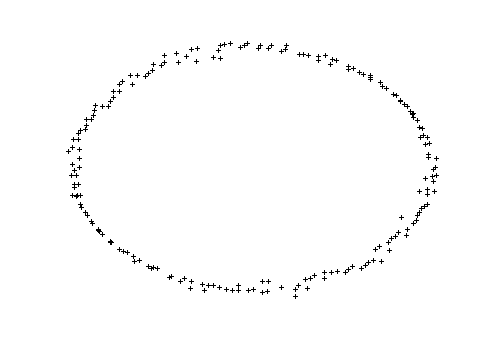
\includegraphics[scale=0.22]{img/ellipse-200-noised-var-1-perimeter}
        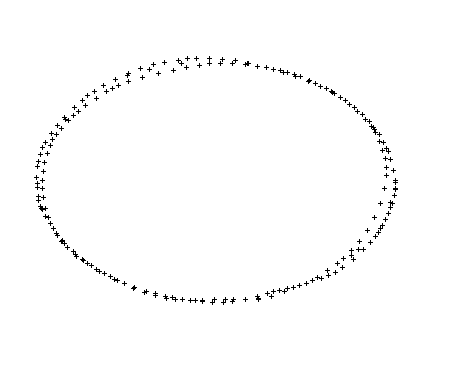
\includegraphics[scale=0.22]{img/ellipse-noised-perimeter-7-2}
        \caption{Aire / Périmètre du bord}
    \end{figure}
\end{frame}

\begin{frame}
    \frametitle{Flot de courbure moyenne}
    % \framesubtitle{Exemples}

    Résultats:
    \begin{itemize}
        \item Aire et périmètre du bord: lissage
        \item Aire: création de trous
    \end{itemize}

    \begin{figure}
        \centering
        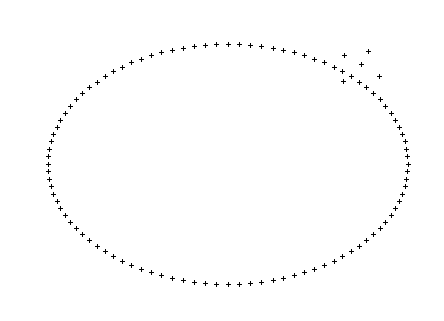
\includegraphics[scale=0.22]{img/ellipse-outliers}
        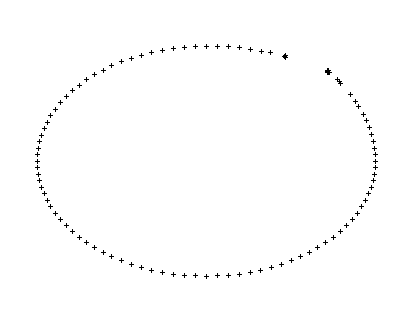
\includegraphics[scale=0.22]{img/ellipse-outliers-area}
        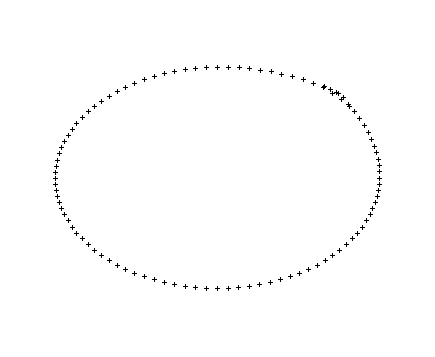
\includegraphics[scale=0.22]{img/ellipse-outliers-perimeter}
        \caption{Nuage de points avec outliers / aire / périmètre du bord}
    \end{figure}
\end{frame}

% {{{1 3D
\section{Cas 3D}

\subsection{Problème}
\begin{frame}
    \frametitle{Problème}
    % \framesubtitle{Flot anisotrope}

    Flot anisotrope:
    \begin{itemize}
        \item Union de polyèdres convexes
        \item Choix du polyèdre $ \to $ influence les directions selon
            lesquelles les points vont être déplacés
    \end{itemize}

    Différentes méthodes:
    \begin{itemize}
        \item Naïve (approchée): intersection cellule de Voronoi et polyèdre
            convexe
        \item Formules d'inclusion-exclusion (approchée)
        \item Arrangements 3D (exacte?)
    \end{itemize}
\end{frame}

\begin{frame}
    \frametitle{Exemples}
    % \framesubtitle{Polyèdres}

    Polyèdres:
    \begin{itemize}
        \item Discrétisation d'une sphère: estimation de normales et courbure
            moyenne
        \item Cube (Norme $ L_{\infty} $)
        \item Bipyramide (Norme $ L_1 $)
    \end{itemize}

    Calcul d'intersection:
    \begin{itemize}
        \item Cellule de Voronoi et polyèdre convexe
        \item Intersection de demi-espaces
        \item Dualité
    \end{itemize}

    \begin{figure}
        \centering
        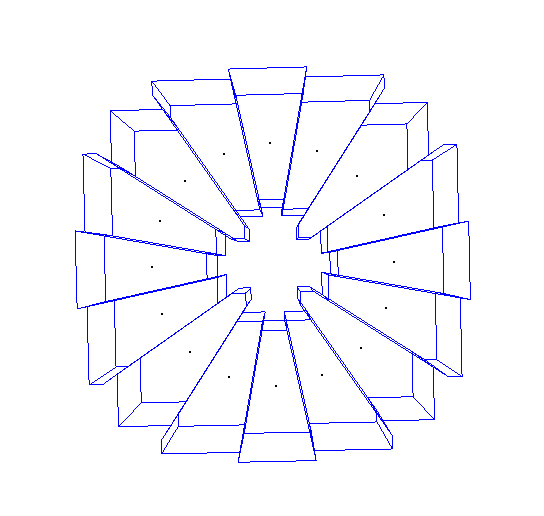
\includegraphics[scale=0.2]{img/circle-cube-inter}
    \end{figure}
\end{frame}

\subsection{Flot anisotrope}
\begin{frame}
    \frametitle{Estimation de normales}
    % \framesubtitle{Exemples}

    Sur une sphère:
    \begin{figure}
        \centering
        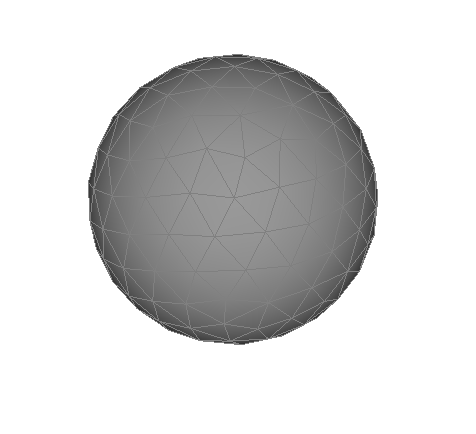
\includegraphics[scale=0.22]{img/sphere-polyhedron-200}
        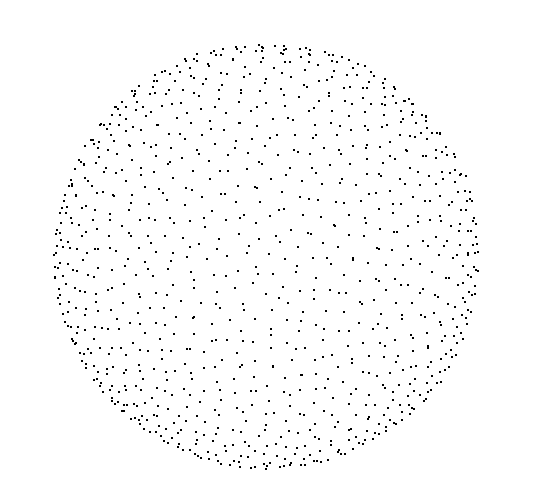
\includegraphics[scale=0.2]{img/sphere-1000}
        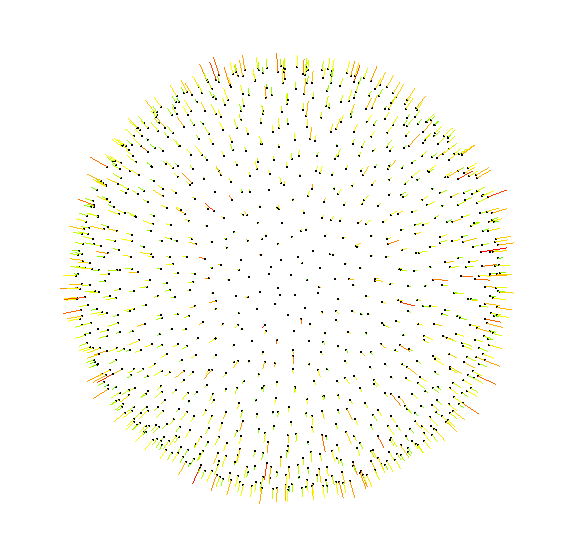
\includegraphics[scale=0.2]{img/sphere-sphere-1000-05}
    \end{figure}
\end{frame}

\begin{frame}
    \frametitle{Flot anisotrope}
    % \framesubtitle{Exemples}

    Cube: 10 itérations
    \begin{figure}
        \centering
        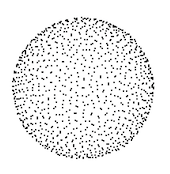
\includegraphics[scale=0.4]{img/sphere-cube-0}
        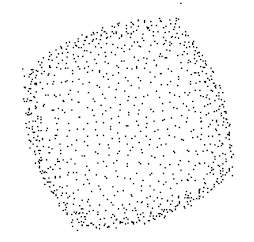
\includegraphics[scale=0.3]{img/sphere-cube-10}
        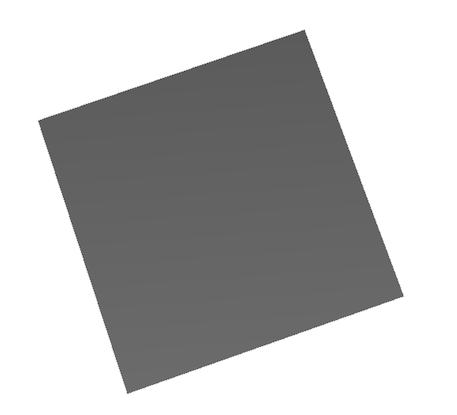
\includegraphics[scale=0.2]{img/sphere-cube-cube}
    \end{figure}

    Bipyramide: 10 itérations
    \begin{figure}
        \centering
        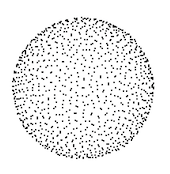
\includegraphics[scale=0.4]{img/sphere-cube-0}
        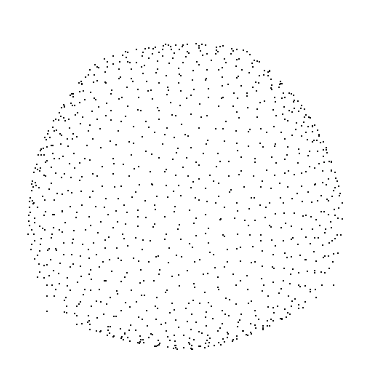
\includegraphics[scale=0.2]{img/sphere-bipyramid-10}
        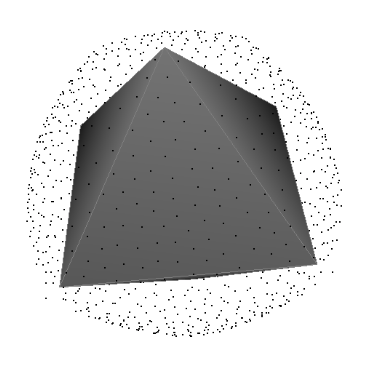
\includegraphics[scale=0.2]{img/sphere-bipyramid-bipyramid}
    \end{figure}
\end{frame}

% {{{1 PERSPECTIVES
\section{Perspectives}

\begin{frame}
    \frametitle{Perspectives}
    % \framesubtitle{Sous-titre}

    \begin{itemize}
        \item Convergence du gradient de l'aire du bord vers la courbure
            moyenne
        \item Compréhension du gradient du flot anisotrope
        \item Tests avec des ellipsoïdes
        \item Amélioration du calcul en 3D (utilisation d'arrangements 3D?)
        \item Simulation de croissance de cristaux (cas anisotrope)
    \end{itemize}
\end{frame}

% \plain{Merci!}
\begin{frame}
    \begin{center}
        \huge{Merci!}
    \end{center}
\end{frame}

\end{document}

% vim: set spelllang=fr :
